\documentclass[11pt,a4paper]{article}
\usepackage[T1]{fontenc}
\usepackage[utf8]{inputenc}
\usepackage{mathpazo}
\usepackage{courier}
\usepackage[margin=25mm]{geometry}
\usepackage{amsmath,amssymb,amsthm,mathtools}
\usepackage{booktabs,array,enumitem}
\usepackage{tikz}
\usetikzlibrary{arrows.meta,positioning}
\usepackage[hidelinks]{hyperref}

\newtheorem{theorem}{Theorem}[section]
\newtheorem{proposition}[theorem]{Proposition}
\newtheorem{corollary}[theorem]{Corollary}
\newtheorem{conjecture}[theorem]{Conjecture}
\theoremstyle{definition}
\newtheorem{definition}[theorem]{Definition}
\newtheorem{question}[theorem]{Open Question}
\theoremstyle{remark}
\newtheorem{remark}[theorem]{Remark}

\newcommand{\Tv}{\mathbf{T}}\newcommand{\Fv}{\mathbf{F}}
\newcommand{\Bv}{\mathbf{B}}\newcommand{\Nv}{\mathbf{N}}
\newcommand{\Bel}{\mathsf{B}}
\newcommand{\pos}[1]{\lVert #1\rVert^{+}}
\newcommand{\negx}[1]{\lVert #1\rVert^{-}}
\newcommand{\lean}[1]{\texttt{\small #1}}
\newcommand{\leqt}{\le_{t}}

\title{Lockean Belief as a Two-Channel Neighbourhood Modality:\\
A Bridge from 4-PEL to Four-Valued Dynamic Epistemic Logic}
\author{J.~L.~Voigt}
\date{Working note, draft 0.2 --- 17 November 2026\\[2pt]
\normalsize Lean~4 artifact: branch \texttt{research/santos-bridge} of
\texttt{cr4bbz/4PEL-Lean-Formalization}}

\begin{document}
\maketitle

\begin{abstract}
\noindent Santos' four-valued dynamic epistemic logic evaluates a relational box over
Belnap--Dunn valued Kripke models and leaves belief as future work. We place the
threshold belief operator of 4-PEL on the same models. Statically, Lockean belief is a
two-channel Scott--Montague neighbourhood modality that validates N, P, M and D and
refutes aggregation~(C); it lies above the relational box in the truth order, and its
support channel coincides with the box exactly in the limit $c=1$ on regular measures,
while the refutation channels differ even there. Dynamically, belief after
conditionalisation reduces to a conditional neighbourhood statement; belief-free
formulas are invariant, belief formulas are not. Santos' state-deleting update can be
adopted in 4-PEL without loss for belief: it is conditionalisation plus pruning of null
worlds, it agrees with conditionalisation on belief in both channels, and it differs
from it on the box. Three gaps of the first draft are closed: with conditional belief
in the language, conditionalisation reduces for \emph{arbitrary} modal depth; adding
Lockean belief is conservative over the box logic of serial relational models with
finite ranges; and aggregation below certainty is replaced by the graded law
$\mu(A\cap B)\ge 2c-1$. All statements marked \emph{proved} are machine-checked in Lean~4
without \texttt{sorry} and without \texttt{native\_decide}. We separate these from
interpretive claims and list the open questions.
\end{abstract}

\section{Introduction}

4-PEL combines Belnap--Dunn values $\{\Tv,\Fv,\Bv,\Nv\}$ \cite{Belnap1977} with a
Lockean threshold: an agent believes $\varphi$ when the mass of the evidence supporting
$\varphi$ reaches a threshold $c>\tfrac12$. Santos \cite{Santos2020} develops a
four-valued epistemic logic on relational models in which agents know about available,
possibly incomplete or conflicting evidence, gives reduction axioms for public
announcements, and explicitly leaves belief open. Evidence models in the sense of van
Benthem and Pacuit \cite{vBP2011} are neighbourhood models; and Kogure \cite{Kogure2025}
recently gave arithmetical completeness results for non-normal logics with neighbourhood
semantics, among them the logic with D but without C. Van Eijck and Renne \cite{vER2014}
axiomatise threshold belief for $c=\tfrac12$ over epistemic neighbourhood models and leave
other thresholds open; probabilistic public announcement logic \cite{vBGK2006} supplies the
reduction axiom that guides Section~\ref{sec:cbel}.

This note asks how the 4-PEL belief operator relates to Santos' box on one and the same
model, and what survives of the dynamic theory. The answer has three parts:
a neighbourhood reading (Section~\ref{sec:nbhd}), a static bridge
(Section~\ref{sec:static}) and a dynamic bridge (Section~\ref{sec:dyn}), completed by
the full reduction law (Section~\ref{sec:cbel}) and a conservativity theorem
(Section~\ref{sec:cons}).
Section~\ref{sec:transfer} states precisely what can and cannot be taken over from
Santos. Section~\ref{sec:open} lists open questions. The appendix maps every numbered
result to its Lean name.

\section{Setting}

A finite 4-PEL model $M=(W,R,\mu,V,c)$ has worlds $W$, accessible ranges $R_i(w)\subseteq W$,
local measures $\mu_{i,w}$ with $\mu_{i,w}(R_i(w))=1$ and $\mu_{i,w}(\emptyset)=0$,
a valuation $V\colon W\times\mathrm{Atom}\to\{\Tv,\Fv,\Bv,\Nv\}$ and thresholds
$\tfrac12<c_i\le 1$. A four-valued proposition is a map $v\colon W\to\{\Tv,\Fv,\Bv,\Nv\}$;
a value is a pair of bits (support, refutation). Inside $R_i(w)$ we write
$\pos{v}$ for the worlds where $v$ is supported and $\negx{v}$ for those where it is refuted.
Belief is
\[
\Bel_i v\,(w) \;=\; \bigl(\ \mu_{i,w}(\pos{v})\ge c_i\ ,\ \ \mu_{i,w}(\negx{v})\ge c_i\ \bigr).
\]
The legacy model interface assumes nothing more about $\mu$. Results that need genuine
probability laws assume \emph{integrity}: nonnegativity, extensionality, monotonicity and
finite additivity on the accessible range. A measure is \emph{regular} at $(i,w)$ if every
accessible world has positive mass.

\section{Belief as a neighbourhood modality}\label{sec:nbhd}

\begin{definition}
The Lockean neighbourhood system is $N_c(w)=\{X\subseteq R(w)\mid \mu_w(X)\ge c\}$.
\end{definition}

\begin{theorem}[two-channel reading; proved]\label{thm:channels}
$\Bel v(w)$ is supported iff $\pos{v}\in N_c(w)$, and refuted iff $\negx{v}\in N_c(w)$.
\end{theorem}

\begin{theorem}[frame laws; proved]\label{thm:frame}
\begin{enumerate}[label=(\alph*),nosep]
\item \textup{(N)} $R(w)\in N_c(w)$ and \textup{(P)} $\emptyset\notin N_c(w)$, for every model.
\item \textup{(M)} Under integrity, $A\subseteq B$ and $A\in N_c(w)$ imply $B\in N_c(w)$.
\item \textup{(D)} Under integrity, disjoint $A,B$ are never both in $N_c(w)$.
\item \textup{($\neg$C)} For three equiprobable worlds and $c=\tfrac23$:
$\{0,1\},\{1,2\}\in N_c$ but $\{1\}\notin N_c$.
\end{enumerate}
\end{theorem}

\begin{corollary}[consistency is a valuation condition; proved]\label{cor:glut}
Under integrity, if no accessible world carries a glut for $v$, then $\Bel v(w)\ne\Bv$.
\end{corollary}

\begin{remark}[asymmetry]\label{rem:asym}
The dual statement fails: a classically valued proposition with mass split $\tfrac12/\tfrac12$
gives $\Bel v=\Nv$. Consistency of belief is controlled by the valuation, completeness by
the concentration of mass. Lockean suspension of judgement exists already in the classical
sector.
\end{remark}

\begin{theorem}[graded aggregation; proved]\label{thm:graded}
Under integrity, for $A,B\subseteq R(w)$: $\mu_w(A\cap B)\ge\mu_w(A)+\mu_w(B)-1$. Hence
$A,B\in N_c(w)$ implies $\mu_w(A\cap B)\ge 2c-1>0$.
\end{theorem}

Theorem~\ref{thm:graded} is what replaces C: the schema
$\Bel_c\varphi\wedge\Bel_c\psi\to\Bel_{2c-1}(\varphi\wedge\psi)$ is sound for the support
channel, it strengthens D, and at $c=1$ it returns aggregation. It is a sound principle
beyond M, N, P, D; we do not claim that it completes the axiomatisation. For
$c=\tfrac12$ a complete system needs a scheme derived from a theorem of Scott
\cite{vER2014}; 4-PEL has $c>\tfrac12$ with a non-strict threshold, which lies in the
range left open there.

\section{The static bridge}\label{sec:static}

\begin{definition}
The relational box is
\[
\Box v(w)=\bigl(\ \forall u\in R(w)\colon v(u)\text{ supported}\ ,\ \
\exists u\in R(w)\colon v(u)\text{ refuted}\ \bigr).
\]
\end{definition}

These are the standard Belnap--Dunn modal clauses. They agree with the clauses Santos
states for $\Diamond$ and $\neg\Diamond$ together with $\neg\Box\varphi\equiv\Diamond\neg\varphi$.

\begin{theorem}[sandwich; proved]\label{thm:sandwich}
For every model and threshold, $\Box v\leqt \Bel v$: a supported box yields supported belief,
and refuted belief yields a refuted box.
\end{theorem}

\begin{theorem}[certainty limit; proved]\label{thm:certainty}
Let $c=1$, assume integrity and regularity at $(i,w)$. Then
\begin{enumerate}[label=(\alph*),nosep]
\item $\Bel v(w)$ is supported iff $\Box v(w)$ is supported;
\item support of belief is closed under conjunction \textup{(C returns)};
\item $\Bel v(w)$ is refuted iff $v$ is refuted at \emph{every} accessible world.
\end{enumerate}
\end{theorem}

\begin{proposition}[strictness; finite witness]\label{prop:strict}
For three equiprobable worlds, $c=\tfrac23$ and $v=(\Tv,\Tv,\Fv)$:
$\Bel v=\Tv$ and $\Box v=\Fv$.
\end{proposition}

Theorem~\ref{thm:certainty}(c) shows that the operators differ even in the limit:
refutation of Lockean belief is universal ($\Box\neg$), refutation of the relational box
is existential ($\Diamond\neg$). Figure~\ref{fig:channels} summarises the static picture.

\begin{figure}[t]
\centering
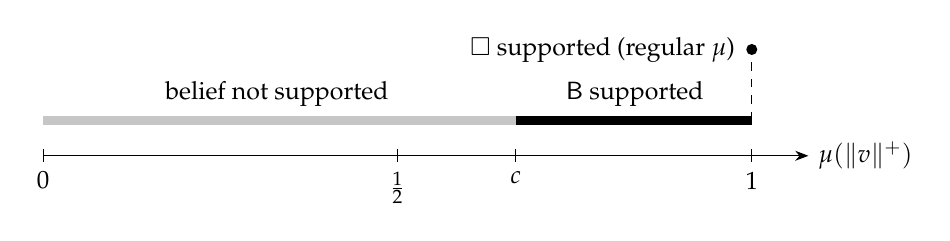
\begin{tikzpicture}[x=9cm,y=1cm,>=Stealth,font=\small]
\draw[->] (0,0)--(1.08,0) node[right]{$\mu(\pos{v})$};
\foreach \x/\l in {0/0,0.5/{\tfrac12},0.6667/{c},1/1}
  \draw (\x,0.08)--(\x,-0.08) node[below]{$\l$};
\draw[line width=3pt,gray!45] (0,0.45)--(0.6667,0.45);
\draw[line width=3pt,black] (0.6667,0.45)--(1,0.45);
\node[above] at (0.33,0.5){belief not supported};
\node[above] at (0.835,0.5){$\Bel$ supported};
\fill (1,1.35) circle (2pt);
\node[left] at (0.99,1.35){$\Box$ supported (regular $\mu$)};
\draw[dashed] (1,0.45)--(1,1.35);
\end{tikzpicture}
\caption{Support channel. The relational box needs all the mass, Lockean belief only the
fraction $c$. The two meet at $c=1$. The refutation channel has the same picture for
$\Bel$ but an existential clause for $\Box$.}\label{fig:channels}
\end{figure}

\section{The dynamic bridge}\label{sec:dyn}

Let $E$ be a formula with $m_E=\mu_w(\pos{E})>0$. 4-PEL \emph{conditionalisation}
$M\!\uparrow\!E$ keeps $R$ and $V$ and replaces $\mu_w(X)$ by $\mu_w(X\cap\pos{E})/m_E$.

\begin{definition}
The conditional neighbourhood system is
$N^{E}_c(w)=\{X\mid \mu_w(X\cap\pos{E})\ge c\cdot \mu_w(\pos{E})\}$.
\end{definition}

\begin{theorem}[reduction; proved]\label{thm:reduction}
For a fixed proposition $v$: after conditionalisation on $E$, $\Bel v(w)$ is supported iff
$\pos{v}\in N^{E}_c(w)$ in the original model, and refuted iff $\negx{v}\in N^{E}_c(w)$.
\end{theorem}

\begin{theorem}[S1: invariance and its limit; proved / finite witness]\label{thm:s1}
\begin{enumerate}[label=(\alph*),nosep]
\item Every belief-free formula has the same value in $M$ and in $M\!\uparrow\!E$.
\item For belief-free $\varphi$, Theorem~\ref{thm:reduction} holds for the formula
$\Bel\varphi$ with $v=[\![\varphi]\!]_M$.
\item Invariance fails for belief formulas: in the model of Figure~\ref{fig:updates},
$\Bel p=\Fv$ before and $\Bel p=\Tv$ after conditionalising on $p$.
\end{enumerate}
\end{theorem}

\subsection*{The Santos update inside 4-PEL}

Santos' announcement deletes the states that do not support the announced formula. The
4-PEL counterpart restricts the accessible range and conditionalises:

\begin{definition}
$M|E$ has $R'(w)=\pos{E}$, $\mu'_w(X)=\mu_w(X\cap\pos{E})/m_E$, and $V$, $c$ unchanged.
\end{definition}

\begin{theorem}[the two updates; proved / finite witness]\label{thm:updates}
\begin{enumerate}[label=(\alph*),nosep]
\item $M|E$ is a 4-PEL model as soon as $m_E\neq 0$ at every $(i,w)$; no further
admissibility condition is needed.
\item Belief-free formulas keep their value in $M|E$.
\item For every proposition $v$, $\Bel v$ has the same value in $M|E$ and in $M\!\uparrow\!E$,
in both channels.
\item The relational box differs: in Figure~\ref{fig:updates}, $\Box p=\Tv$ in $M|p$ but
$\Box p=\Fv$ in $M\!\uparrow\!p$, although $\Bel p=\Tv$ in both.
\end{enumerate}
\end{theorem}

\begin{figure}[t]
\centering
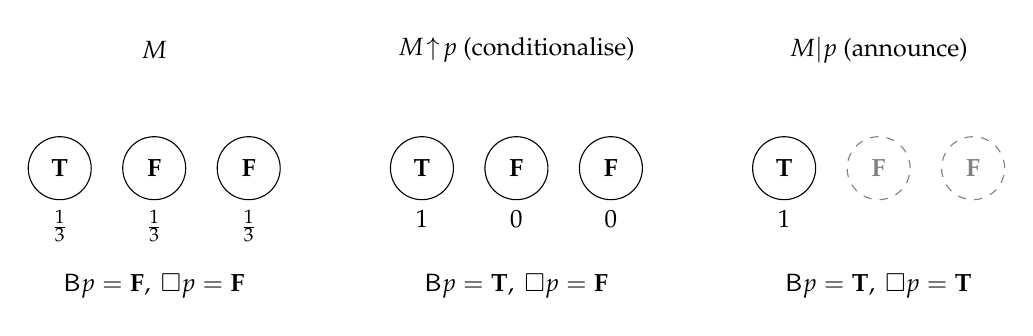
\begin{tikzpicture}[font=\small,>=Stealth,
  w/.style={circle,draw,minimum size=8mm,inner sep=0pt},
  dead/.style={circle,draw,dashed,gray,minimum size=8mm,inner sep=0pt}]
\begin{scope}
\node at (1.2,1.5){$M$};
\node[w,label=below:{$\tfrac13$}] (a0) at (0,0){$\Tv$};
\node[w,label=below:{$\tfrac13$}] (a1) at (1.2,0){$\Fv$};
\node[w,label=below:{$\tfrac13$}] (a2) at (2.4,0){$\Fv$};
\node at (1.2,-1.5){$\Bel p=\Fv,\ \Box p=\Fv$};
\end{scope}
\begin{scope}[xshift=4.6cm]
\node at (1.2,1.5){$M\!\uparrow\! p$ (conditionalise)};
\node[w,label=below:{$1$}] (b0) at (0,0){$\Tv$};
\node[w,label=below:{$0$}] (b1) at (1.2,0){$\Fv$};
\node[w,label=below:{$0$}] (b2) at (2.4,0){$\Fv$};
\node at (1.2,-1.5){$\Bel p=\Tv,\ \Box p=\Fv$};
\end{scope}
\begin{scope}[xshift=9.2cm]
\node at (1.2,1.5){$M|p$ (announce)};
\node[w,label=below:{$1$}] (c0) at (0,0){$\Tv$};
\node[dead] (c1) at (1.2,0){$\Fv$};
\node[dead] (c2) at (2.4,0){$\Fv$};
\node at (1.2,-1.5){$\Bel p=\Tv,\ \Box p=\Tv$};
\end{scope}
\end{tikzpicture}
\caption{Three equiprobable worlds, $c=\tfrac23$, atom $p$ with values
$(\Tv,\Fv,\Fv)$. Conditionalisation keeps the null worlds accessible; the Santos update
removes them from the range. Belief agrees, the box does not.}\label{fig:updates}
\end{figure}

\begin{remark}\label{rem:regular}
In $M\!\uparrow\!p$ the measure is no longer regular, so the hypothesis of
Theorem~\ref{thm:certainty} fails: an agent can believe with full mass and still not have
a supported box. $M|p$ removes exactly the null worlds that cause this.
\end{remark}

\section{Conditional belief and the full reduction law}\label{sec:cbel}

Probabilistic public announcement logic reduces
$[!A]P(\varphi)=k$ to $A\to P([!A]\varphi\mid A)=k$ \cite{vBGK2006}: the announcement is
pushed inside, and the static language needs conditional probability. We follow this
pattern. The extended language adds conditional belief $\Bel(\varphi\mid\psi)$ and the
relational box to atoms, $\neg$, $\wedge$ and $\Bel$, with
\[
\Bel(\varphi\mid\psi)(w)=\bigl(\ \mu_w(\pos{\varphi}\cap\pos{\psi})\ge c\,\mu_w(\pos{\psi})\ ,\ \
\mu_w(\negx{\varphi}\cap\pos{\psi})\ge c\,\mu_w(\pos{\psi})\ \bigr).
\]
The reduct $\mathrm{red}_E$ is defined by recursion: it commutes with atoms, $\neg$,
$\wedge$ and $\Box$, and
\[
\mathrm{red}_E(\Bel\varphi)=\Bel(\mathrm{red}_E\varphi\mid E),\qquad
\mathrm{red}_E(\Bel(\varphi\mid\psi))=\Bel(\mathrm{red}_E\varphi\mid \mathrm{red}_E\psi\wedge E).
\]

\begin{theorem}[full reduction; proved]\label{thm:fullred}
If $\mu_{i,w}(\pos{E})>0$ for all $(i,w)$, then for every formula $\varphi$ of the extended
language and every world $w$:
$\ [\![\varphi]\!]_{M\uparrow E}(w)=[\![\mathrm{red}_E\,\varphi]\!]_{M}(w)$.
\end{theorem}

This holds for arbitrary modal depth and as an identity of four-valued values, not only
of support. It settles the nesting question for conditionalisation and confirms that
conditional belief is the right static primitive: the language with $\Bel(\cdot\mid\cdot)$
is closed under the update. By convention a condition of mass zero makes conditional
belief both supported and refuted. For the state-deleting update $M|E$ the belief clauses
are the same (Theorem~\ref{thm:updates}c); the box would need a relativised clause and is
not covered.

\section{Conservativity over the relational box logic}\label{sec:cons}

A relational model $S=(R,V)$ has finite accessible ranges and a four-valued valuation; it
is serial if no range is empty. Box formulas are built from atoms, $\neg$, $\wedge$, $\Box$.

\begin{theorem}[conservativity; proved]\label{thm:cons}
\begin{enumerate}[label=(\alph*),nosep]
\item Every 4-PEL model is serial, and a box formula has the same value in a 4-PEL model
and in its relational reduct.
\item Every serial relational model expands to a 4-PEL model (uniform counting measure on
each range) whose reduct it is.
\item For every property $D$ of values: a box formula has $D$ at every world of every
4-PEL model iff it has $D$ at every world of every serial relational model.
\end{enumerate}
\end{theorem}

Taking $D$ to be ``supported'' or ``not refuted'' gives conservativity for either notion
of validity; the same argument applies to consequence. The statement is relative to
serial models with finite ranges, which is what 4-PEL models are. It becomes a statement
about Santos' logic once his box clause is confirmed to be the one used here and his logic
is restricted to serial frames; if that logic has the finite model property, finiteness is
no restriction.

\section{What transfers from Santos, and what does not}\label{sec:transfer}

\paragraph{Transfers without loss (proved).}
The state-deleting update is definable in 4-PEL with a single proof obligation
(Theorem~\ref{thm:updates}a). For belief it is \emph{equivalent} to conditionalisation
(Theorem~\ref{thm:updates}c), so every existing 4-PEL result about belief under
conditionalisation holds verbatim for the Santos update. Atoms, negation and conjunction
are invariant under both updates (Theorems~\ref{thm:s1}a, \ref{thm:updates}b), which is
the content of Santos' reduction clauses for the propositional connectives.

\paragraph{Does not transfer unchanged.}
(i)~The reduction clause for the box cannot be used for belief: after the update, belief
is a statement about a \emph{conditional} neighbourhood (Theorem~\ref{thm:reduction}), and
a threshold can be crossed in either direction (Theorem~\ref{thm:s1}c).
(ii)~The refutation clause differs in kind (Theorem~\ref{thm:certainty}c).
(iii)~Aggregation is unavailable below certainty (Theorem~\ref{thm:frame}d), so any
argument that uses normality of the modality is lost.

\paragraph{Interpretive, not machine-checked.}
(a)~The identification of our box with Santos' $\Box$ rests on the standard clauses and
on the clauses the paper states for $\Diamond$; the displayed definition should be checked
against the published text before it is cited by number.
(b)~Santos deletes states globally; $M|E$ restricts each accessible range and keeps the
set of worlds. For formulas of modal depth at most one the two coincide by construction;
for nested modalities the comparison is open (Question~\ref{q:nested}).
(c)~Conservativity is now a theorem (Theorem~\ref{thm:cons}), but over serial relational
models with finite ranges and the box clauses used here; its transfer to Santos' own
system depends on (a), on seriality, and on the finite model property of his logic, none
of which is machine-checked.

\section{Open questions}\label{sec:open}

\begin{question}[reduction for the state-deleting update]\label{q:nested}
Theorem~\ref{thm:fullred} covers conditionalisation. For $M|E$ the box needs a relativised
clause, and global state deletion has to be compared with range restriction for nested
modalities.
\end{question}

\begin{question}[definability of conditional belief]
Is $\Bel(\varphi\mid E)$ definable from $\Bel$ and the connectives? We conjecture that it
is not; Theorem~\ref{thm:fullred} shows only that it suffices.
\end{question}

\begin{question}[frame laws under update]
Which of N, P, M, D hold for $N^{E}_c$? N and P are expected for $m_E>0$, D for events
that are disjoint inside $\pos{E}$.
\end{question}

\begin{question}[the refutation channel]
Is a second primitive $\neg\Bel\neg$ needed to express the existential refutation of the
relational box?
\end{question}

\begin{question}[threshold crossing]
Characterise when $\Bel\varphi$ and $[E]\Bel\varphi$ differ in terms of
$\mu(\pos{\varphi}\cap\pos{E})/\mu(\pos{E})$ and $\mu(\pos{\varphi})$, and relate this to
the existing instability and restoration results of 4-PEL.
\end{question}

\begin{question}[axiomatisation]
Which system is complete for $N_c$ at a fixed $c\in(\tfrac12,1)$ with a non-strict
threshold? M, N, P, D and graded aggregation are sound; for $c=\tfrac12$ completeness
needs a Scott-type scheme and a certainty operator \cite{vER2014}. We make no
completeness claim.
\end{question}

\appendix
\section{Correspondence with the Lean artifact}

All listed theorems depend only on \lean{propext}, \lean{Classical.choice} and
\lean{Quot.sound}. Status: P = proved in general, W = finite witness.

\medskip
{\footnotesize\renewcommand{\lean}[1]{\texttt{#1}}\noindent\begin{tabular}{@{}l>{\raggedright\arraybackslash}p{0.72\textwidth}c@{}}
\toprule
Result & Lean name (namespace \lean{PEL4}) & Status\\
\midrule
Thm.~\ref{thm:channels} & \lean{belief\_pos\_iff\_neighbourhood}, \lean{belief\_neg\_iff\_neighbourhood} & P\\
Thm.~\ref{thm:frame}a & \lean{neighbourhood\_N}, \lean{neighbourhood\_P} & P\\
Thm.~\ref{thm:frame}b,c & \lean{neighbourhood\_M}, \lean{neighbourhood\_D} & P\\
Thm.~\ref{thm:frame}d & \lean{neighbourhood\_not\_C} & W\\
Cor.~\ref{cor:glut} & \lean{belief\_thresholdConsistent\_of\_no\_glut} & P\\
Thm.~\ref{thm:graded} & \lean{mass\_intersection\_lower\_bound}, \lean{neighbourhood\_graded\_C}, \lean{neighbourhood\_intersection\_pos} & P\\
Thm.~\ref{thm:sandwich} & \lean{santosBox\_pos\_implies\_belief\_pos}, \lean{belief\_neg\_implies\_santosBox\_neg} & P\\
Thm.~\ref{thm:certainty}a & \lean{belief\_pos\_eq\_santosBox\_pos\_of\_certainty} & P\\
Thm.~\ref{thm:certainty}b & \lean{belief\_pos\_and\_of\_certainty} & P\\
Thm.~\ref{thm:certainty}c & \lean{belief\_neg\_iff\_all\_neg\_of\_certainty} & P\\
Prop.~\ref{prop:strict} & \lean{belief\_T\_but\_santosBox\_F} & W\\
Thm.~\ref{thm:reduction} & \lean{belief\_conditionalize\_pos\_iff}, \lean{belief\_conditionalize\_neg\_iff} & P\\
Thm.~\ref{thm:s1}a & \lean{eval\_conditionalize\_of\_beliefFree} & P\\
Thm.~\ref{thm:s1}b & \lean{eval\_bel\_conditionalize\_pos\_iff}, \lean{eval\_bel\_conditionalize\_neg\_iff} & P\\
Thm.~\ref{thm:s1}c & \lean{bel\_not\_invariant} & W\\
Thm.~\ref{thm:updates}a & \lean{announce} (definition with proof fields) & P\\
Thm.~\ref{thm:updates}b & \lean{eval\_announce\_of\_beliefFree} & P\\
Thm.~\ref{thm:updates}c & \lean{belief\_announce\_eq\_conditionalize} & P\\
Thm.~\ref{thm:updates}d & \lean{box\_announce\_ne\_conditionalize} & W\\
Thm.~\ref{thm:fullred} & \lean{evalC\_condOn\_eq\_red} (with \lean{CFormula}, \lean{condBelief}, \lean{red}) & P\\
Thm.~\ref{thm:cons}a & \lean{Model.reduct\_serial}, \lean{evalC\_toC\_eq\_evalR} & P\\
Thm.~\ref{thm:cons}b & \lean{RelModel.expand}, \lean{RelModel.reduct\_expand}, \lean{evalC\_expand\_eq\_evalR} & P\\
Thm.~\ref{thm:cons}c & \lean{box\_validity\_conservative} & P\\
\bottomrule
\end{tabular}}

\medskip
\sloppy\noindent Remark~\ref{rem:asym} is covered by the existing theorem
\lean{gate6BeliefBoundary\_not\_thresholdComplete} only as far as that theorem's own
statement goes; the $\tfrac12/\tfrac12$ example is given here informally.
Remark~\ref{rem:regular} is an observation about the witness model and is not a separate
Lean theorem. The Lean modules and this draft were prepared with the assistance of Claude.

\begin{thebibliography}{9}
\bibitem{Belnap1977} N.~D. Belnap. A useful four-valued logic. In J.~M. Dunn and
G.~Epstein (eds.), \emph{Modern Uses of Multiple-Valued Logic}, Reidel, 1977.
\bibitem{vBP2011} J.~van Benthem and E.~Pacuit. Dynamic logics of evidence-based beliefs.
\emph{Studia Logica} 99, 2011. (ILLC Prepublication PP-2011-19.)
\bibitem{Kogure2025} H.~Kogure. Provability interpretation of non-normal modal logics
having neighborhood semantics. arXiv:2511.16488, 2025.
\bibitem{vBGK2006} J.~van Benthem, J.~Gerbrandy and B.~Kooi. Dynamic update with
probabilities. ILLC Prepublication, 2006.
\bibitem{vER2014} J.~van Eijck and B.~Renne. Belief as willingness to bet.
arXiv:1412.5090, 2014.
\bibitem{Santos2020} Y.~D. Santos. A four-valued dynamic epistemic logic.
\emph{Journal of Logic, Language and Information} 29:451--489, 2020.
\end{thebibliography}
\end{document}
